\chapter[Boundary Conditions]{Boundary and Initial Conditions, and Some Other Transport Equations}

The last lecture introduced both general transport equations and the neutron transport equation.  In this lecture, we discuss several boundary and interface conditions for constraining the transport equation.  We finish by briefly describing two additional transport equations that help us recognize special features of the neutron transport equation.

\section*{Boundary and Initial Condtions}

In the last lacture, we finished with the Eq. \ref{eq:neutrontransport} neutron transport equation:
\begin{equation*}
  \begin{split}
     \frac{1}{v}\frac{\partial \psi}{\partial t} &+ \hat{\Omega} \cdot \nabla \psi + \Sigma_t \psi(\mathbf{r},\mathbf{\Omega},E,t) = \\
           &+ \int^{\infty}_{0} dE' \int_{4\pi} d\Omega' \Sigma_s(\mathbf{r},\mathbf{\Omega}\cdot\mathbf{\Omega}',E'\to E)\psi(\mathbf{r},\mathbf{\Omega'},E',t) +s \, .
  \end{split}
\end{equation*}
This is an integro-differential equation in 7 variables: 3 in space, 2 in angle, 1 in energy, and time.  Like all differential equations, the transport equation requires initial and boundary conditions. 

\subsection*{Initial Conditions}

Initial conditions for the transport equation are relatively straightforward.  At some initial time $t_0$, an initial condition is expressed as
\begin{equation}
 \psi(\mathbf{r},\mathbf{\Omega},E,t)|_{t=t_0} = f(\mathbf{r},\mathbf{\Omega},E) \, ,
\end{equation}
where $f$ represents a known function of space, angle, and energy.  

Time-dependent problems in neutron transport are often quite challenging due to the wide range of time scales involved.  A good example comes from the study of reactor kinetics, where the time scales range from prompt neutron lifetimes (on the order of 10$^{-5}$ seconds) to the delayed neutrons of longest lifetime (on the order of tens of seconds).  Any numerical scheme is effectively limited by the smallest time scale, leading to a ``stiff'' problem.  

Other neutron transport problems exhibit even more diverse time scales.  The time scale for nuclear weapons is perhaps most easily quantified with ``shakes'', that is 10$^{-8}$ seconds.  Isotopic changes in nuclear reactors due to irradiation can have profound effects on time scales ranging from hours (xenon production) up to months or years (burnup).

Frequently, we are interested in steady state values, so that $\frac{\partial \psi}{\partial t} = 0$.  If the source $s$ in Eq. \ref{eq:neutrontransport} includes an external source, then the problem is a \textit{fixed source problem}.  If $s$ does not include an external source (and includes only e.g. a fission source), then the problem becomes an \textit{eigenvalue problem}, which are studied in Lecture \ref{lec:criticality}.

\subsection*{Boundary Conditions}

The most straightforward boundary condition to enforce is the \textit{free surface} or \textit{vacuum} condition.  Physically, the condition represents the situation where no neutrons enter a volume from the outside.  In other words, the volume of interest can be thought to exist in a void.  Mathematically, the condition is expressed
\begin{equation}
 \psi(\mathbf{r},\mathbf{\Omega},E,t) = 0 \, , \, \, \, \,  \, \, \, \mathbf{\hat{n}} \cdot \mathbf{\Omega} < 0 \, ,
\end{equation}
where $\mathbf{\hat{n}}$ is the unit \textit{outward normal} vector to the surface of interest.  
% is there a better way to give nice wrapping??  
\begin{wrapfigure}{r}{0.3\textwidth}
    \begin{center}
    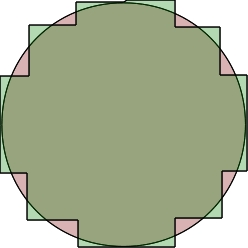
\includegraphics[keepaspectratio, width = 1.25 in]{squarecylinder}
    \end{center}
    \caption{A reentrant square cyclinder.}
    \label{fig:squarecylinder}
\end{wrapfigure}
Since $\mathbf{\hat{n}} \cdot \mathbf{\Omega}$ is just the cosine of the angle between the incident neutrons and the normal vector, we see the flux vanishes whenever that cosine is negative, or whenever the neutron direction is inward.

A point of warning: reentrant geometries must be avoided when using vacuum conditions.  Unless treated with special care, reentrant geometries lead to inconsistency.  Neutrons leaving one portion of the geometry could, in theory, reenter another portion, but since vacuum conditions disallow this, the true problem is not modeled correctly.  A common example of this occurs when ``squaring'' an exterior cylindrical boundary, as exhibited in Figure \ref{fig:squarecylinder}.

Another useful boundary condition is simply to specify the incident flux when it is known:
\begin{equation}
 \psi(\mathbf{r}_s,\mathbf{\Omega},E,t) = f(\mathbf{r}_s,\mathbf{\Omega},E,t) \, .
\end{equation}
In this way, boundary sources can be defined.

A \textit{reflective} or \textit{specular} condition is such that 
\begin{equation}
 \psi(\mathbf{r}_s,\mathbf{\Omega},E,t) = \psi(\mathbf{r}_s,\mathbf{\Omega}_R,E,t) \, , \, \, \, \,  \, \, \, \mathbf{\hat{n}} \cdot \mathbf{\Omega} < 0 \, ,
\end{equation}
where $\mathbf{\Omega}_R$ is the (mirror) reflection of $\mathbf{\Omega}$.  Reflective conditions are widely used in lattice physics, where pin cells or assemblies are modeled in an infinite array; the ``infinite'' is captured by the reflective conditions.  See Figure \ref{fig:reflectiveperiodic}.

A variation on reflective conditions is an \textit{albedo} condition, where
\begin{equation}
 \psi(\mathbf{r}_s,\mathbf{\Omega},E,t) = \alpha \psi(\mathbf{r}_s,\mathbf{\Omega}_R,E,t) \, , \, \, \, \,  \, \, \, \mathbf{\hat{n}} \cdot \mathbf{\Omega} < 0 \, .
\end{equation}
Here, $\alpha$ is the ``albedo'' and quantifies the strength with which neutrons stream back into the system after streaming out.  Historically, albedo conditions were highly useful since they can often capture the physics of reflectors with minimum computational cost.  The albedos for many materials were precomputed (or found experimentally), effectively eliminating a significant portion of phase space in e.g. reactor analysis.

Another approach is to use \textit{periodic} conditions, such that
\begin{equation}
 \psi(\mathbf{r}_1,\mathbf{\Omega},E,t) = \psi(\mathbf{r}_2,\mathbf{\Omega},E,t) \, ,
\end{equation}
Figure \ref{fig:reflectiveperiodic} illustrates both reflective and periodic boundary conditions.  Periodic conditions work well in infinite arrays that have assymetric unit cells (for which reflective conditions would represent an infinite but incorrect array).

\begin{figure}[h] 
    \centering
    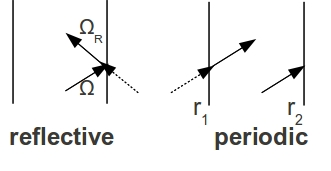
\includegraphics[keepaspectratio, width = 2.0 in]{reflectiveperiodic}
    \caption{Reflective and periodic boundary conditions.}
    \label{fig:reflectiveperiodic}
\end{figure}

The final boundary condition we mention is the \textit{white boundary condition}, a condition where all neutrons incident on a boundary reflect back isotropically in angle.  For this case,
\begin{equation}
\begin{split}
 \psi(\mathbf{r}_s,\mathbf{\Omega},E,t) &= \frac{ \int_{\mathbf{\hat{n}} \cdot \mathbf{\Omega}' > 0}   \mathbf{\hat{n}} \cdot \mathbf{\Omega}' \psi (\mathbf{r},\mathbf{\Omega}',E,t)d\Omega' } {  \int_{\mathbf{\hat{n}} \cdot \mathbf{\Omega}' > 0}  \mathbf{\hat{n}} \cdot \mathbf{\Omega}'  d\Omega'    }  \\
             &= \frac{ J_+ (\mathbf{r}_s,E,t) } {  \int_{\mathbf{\hat{n}} \cdot \mathbf{\Omega}' > 0}  \mathbf{\hat{n}} \cdot \mathbf{\Omega}'  d\Omega'    }\, , \, \, \, \,  \, \, \, \mathbf{\hat{n}} \cdot \mathbf{\Omega}' < 0 \, .
\end{split}
\end{equation}
Note the conditions on $\mathbf{\Omega}$ and $\mathbf{\Omega}'$.  The first corresponds to the left hand side and is limited to $\mathbf{\hat{n}} \cdot \mathbf{\Omega}' < 0$, i.e. incoming directions.  Contrarily, $\mathbf{\Omega}'$ is the dummy variable on the right hand side, and is always integrated over the domain where $\mathbf{\hat{n}} \cdot \mathbf{\Omega}' > 0$, i.e. outgoing directions.  This is so because we integrate the entire outgoing neutron population (which is proportional to the outgoing partial current) and then redistribute that number uniformly over all incident directions, i.e. isotropically.

White boundary conditions have had use in lattice physics where an isotropic angular distribution is sometimes relatively accurate.  In particular, the white boundary condition provides a useful fix for reflective conditions in Wigner-Seitz cells, which convert square pin cells into equivalent cylindrical cells, since cylindrical cells can be treated with 1-d methods.  However, while in square cells the reflective conditions work fine, they do not work well in cylindrical geometries (see Figure \ref{fig:wignerseitz}), since neutrons entering at certain angles can spend too much time in the moderator before colliding.  This consequently leads to overprediction of the moderator flux, an artifact known as the Newmarch effect. As a result, white conditions are used.


\begin{figure}[h] 
    \centering
    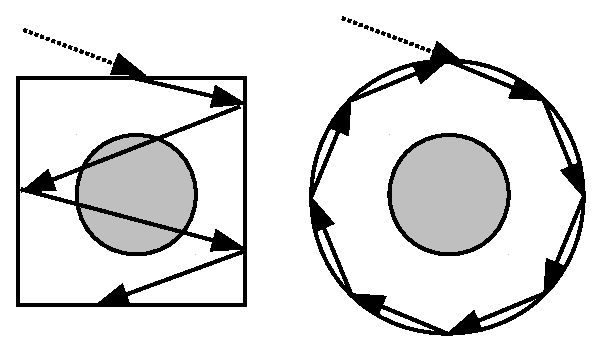
\includegraphics[keepaspectratio, width = 3.0 in]{wignerseitz}
    \caption{Square pin cell and equivalent Wigner-Seitz cell.  Same incident direction and location.}
    \label{fig:wignerseitz}
\end{figure}

\section*{Other Transport Equations}

We finish this lecture by presenting in brief two other important transport equations.

\subsection*{Photon Transport}

Photon transport is fundamental to radiation hydrodynamics (an integral aspect of ``bomb'' physics) and astrophysics.  Photon transport can largely be divided into two classes of problems: \textit{radiative transfer}, which consists of the propogation of soft (low energy) x-rays, and \textit{high energy} photon transport, which can largely be treated as we do neutrons.  We briefly describe the former.

The quantity of interest is the intensity, essentially an ``energy angular flux'', and is defined
\begin{equation}
 I_{\nu}(\mathbf{r},\mathbf{\Omega},t) = (h\nu)cn(\mathbf{r},\mathbf{\Omega},E,t) \, ,
\end{equation}
where $h\nu$ is the photon energy.  The ``radiative transfer equation'' is
\begin{equation}
 \frac{1}{c}\frac{\partial I_{\nu}}{\partial t} + \Omega \cdot \nabla I_{\nu} = \rho(\varepsilon_{\nu} - \kappa_{\nu}I_{\nu}) \, ,
 \label{eq:radiative}
\end{equation}
where $\varepsilon$ is a mass emission coefficient (a source term), and $\kappa$ is a mass attenuation coefficient (a loss term).  The radiative transfer equations are nonlinear due to the temperature-dependence of the underlying interaction coefficients (the ``cross-sections), particularly the emission term (which is not explicitly represented in Eq. \ref{eq:radiative}).

For the case of local thermodynamic equilibrium (LTE), Eq. \ref{eq:radiative} is simplified somewhat.  Local thermodynamic equilibrium exists when the quantity $S_{\nu} = \varepsilon_{\nu}/\kappa_{\nu} = B_{\nu}$, where $B_{\nu}$ is the Planck distribution (i.e. the black body spectrum).  In this case, Eq. \ref{eq:radiative} takes the form
\begin{equation}
 \frac{1}{c}\frac{\partial I_{\nu}}{\partial t} + \Omega \cdot \nabla I_{\nu} = \rho \kappa_{\nu} (B_{\nu} - I_{\nu}) \, .
 \label{eq:radiativelte}
\end{equation}

Radiative transfer is inherently a frequency-dependent process: the coefficients depend on the frequency, and a medium emits photons of a wide range of frequencies.  A frequently used approximation is to neglect this dependence in what is called the \textit{grey approximation}, similar to the one-speed studies in neutron transport we will study in the next several lectures.  ``Black bodies'' are also often used; these are pure absorbers whose emission spectrum is the Planck distribution.

To determine the temperature (dependence on which is implicit in all the quantities of Eq. \ref{eq:radiative}), an energy conservation equation is used.  As an example, using the grey approximation and assuming temperature- and spatially-independent coefficients, Eq. \ref{eq:radiative} becomes
\begin{equation}
 \frac{1}{c}\frac{\partial I}{\partial t} + \Omega \cdot \nabla I(\mathbf{r},\mathbf{\Omega},t) = \rho \kappa (acT^4(\mathbf{r},t)- I) \, ,
 \label{eq:radiativegrey}
\end{equation}
where $a$ is the emissivity (as in the Stefan-Boltzmann law) and $T$ is the temperature.  The corresponding energy conservation equation is
\begin{equation}
 \overbrace{c_v \frac{\partial T}{\partial t}}^{\text{energy rate of change}} = \overbrace{\rho \kappa}^{\text{abs. coef.}} \overbrace{\int_{4\pi} I(\mathbf{r},\mathbf{\Omega},t) d\Omega}^{\text{energy flux}} - \overbrace{\rho \kappa a c T^4(\mathbf{r},t)}^{\text{loss due to emission}} + \overbrace{Q(\mathbf{r},t)}^{\text{gains from outside}} \, ,
\end{equation}
where $c_v$ is the specific heat and $Q$ represents any external energy source.


\subsection*{Plasma Transport}

Another area of interest for nuclear engineers is plasma physics.  Let us apply Eq. \ref{eq:generalte} to electrons in a plasma, where we substitute in the Lorentz force for $\mathbf{F}$:
\begin{equation}
  \frac{\partial n}{\partial t} 
   + \mathbf{v} \cdot \nabla n + \frac{e}{m} \Big ( \mathbf{E}+(\mathbf{v}\times \mathbf{B} ) \Big ) \cdot \nabla_{\mathbf{v}} n =   \Big( \frac{\partial n}{\partial t} \Big )_{\mathrm{coll}} +  s \, .
\end{equation}
If we neglect sources and collisions, we arrive at the Vlasov equation:
\begin{equation}
  \frac{\partial n}{\partial t} 
   + \mathbf{v} \cdot \nabla n + \frac{e}{m} \Big ( \mathbf{E}+(\mathbf{v}\times \mathbf{B} ) \Big ) \cdot \nabla_{\mathbf{v}} n =  0 \, .
\end{equation}
Augmented with Maxwell's equations, the Vlasov equation gives a rather complete description of collisionless plasmas.  

\section*{Further Reading}

The treatment of boundary conditions is rather straightforward, but the student may wish to consult e.g. Duderstadt and Martin \cite{duderstadt1976tt} or Lewis and Miller \cite{lewis1993cmn}.  The discussion of white boundary conditions and the Wigner-Seitz dilemma follows that of H\'{e}bert \cite{hebert2009arp}, and the Newmarch effect is identified by Stamm'ler and Abbate \cite{stammler1983mss}.   

The discussion of photon and plasma transport largely follows that of Duderstadt and Martin \cite{duderstadt1976tt}.  The example grey approximation equations are given in a paper by Miller and Lewis \cite{miller1987nrm}, and there is a wealth of literature on the subject.  For those interested in radiative transfer as it applies to atmospheres, see MIT course 12.815.



